\documentclass{minimal}
\usepackage{bm}
\usepackage{epsfig,color}
\usepackage[papersize={576.00bp,432.00bp},text={576.00bp,432.00bp}]{geometry}
\begin{document}
\centering
% Title: glps_renderer figure
% Creator: GL2PS 1.3.8, (C) 1999-2012 C. Geuzaine
% For: Octave
% CreationDate: Fri Aug 14 13:54:44 2015
\setlength{\unitlength}{1pt}
\begin{picture}(0,0)
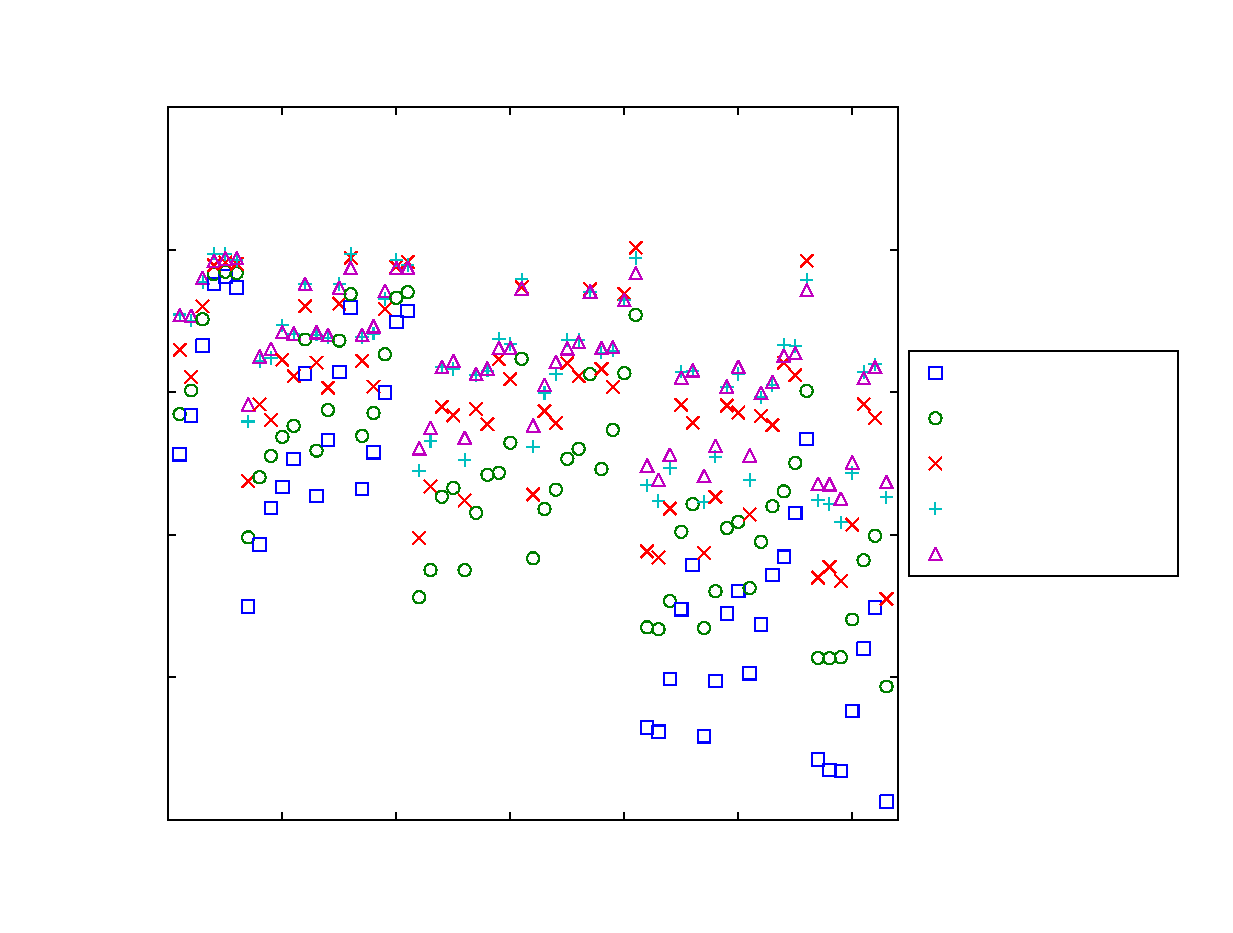
\includegraphics{dEE-inc}
\end{picture}%
\begin{picture}(576,432)(0,0)
\fontsize{16}{0}
\selectfont\put(72.8,41.1956){\makebox(0,0)[t]{\textcolor[rgb]{0,0,0}{{0}}}}
\fontsize{16}{0}
\selectfont\put(127.513,41.1956){\makebox(0,0)[t]{\textcolor[rgb]{0,0,0}{{10}}}}
\fontsize{16}{0}
\selectfont\put(182.225,41.1956){\makebox(0,0)[t]{\textcolor[rgb]{0,0,0}{{20}}}}
\fontsize{16}{0}
\selectfont\put(236.938,41.1956){\makebox(0,0)[t]{\textcolor[rgb]{0,0,0}{{30}}}}
\fontsize{16}{0}
\selectfont\put(291.651,41.1956){\makebox(0,0)[t]{\textcolor[rgb]{0,0,0}{{40}}}}
\fontsize{16}{0}
\selectfont\put(346.363,41.1956){\makebox(0,0)[t]{\textcolor[rgb]{0,0,0}{{50}}}}
\fontsize{16}{0}
\selectfont\put(401.076,41.1956){\makebox(0,0)[t]{\textcolor[rgb]{0,0,0}{{60}}}}
\fontsize{16}{0}
\selectfont\put(67.7977,46.2){\makebox(0,0)[r]{\textcolor[rgb]{0,0,0}{{-4}}}}
\fontsize{16}{0}
\selectfont\put(67.7977,114.66){\makebox(0,0)[r]{\textcolor[rgb]{0,0,0}{{-3}}}}
\fontsize{16}{0}
\selectfont\put(67.7977,183.12){\makebox(0,0)[r]{\textcolor[rgb]{0,0,0}{{-2}}}}
\fontsize{16}{0}
\selectfont\put(67.7977,251.58){\makebox(0,0)[r]{\textcolor[rgb]{0,0,0}{{-1}}}}
\fontsize{16}{0}
\selectfont\put(67.7977,320.04){\makebox(0,0)[r]{\textcolor[rgb]{0,0,0}{{0}}}}
\fontsize{16}{0}
\selectfont\put(67.7977,388.5){\makebox(0,0)[r]{\textcolor[rgb]{0,0,0}{{1}}}}
\fontsize{16}{0}
\selectfont\put(247.881,28.1956){\makebox(0,0)[t]{\textcolor[rgb]{0,0,0}{{\textbf{cluster}}}}}
\fontsize{16}{0}
\selectfont\put(53.7977,217.35){\rotatebox{90}{\makebox(0,0)[b]{\textcolor[rgb]{0,0,0}{{$E^+_{clust} - E^0_{clust} - E^+_{H_5O_2+} + E^0_{H_4O_2}$ [eV]}}}}}
\fontsize{16}{0}
\selectfont\put(453.661,260.689){\makebox(0,0)[l]{\textcolor[rgb]{0,0,0}{{nwchem}}}}
\fontsize{16}{0}
\selectfont\put(453.661,239.02){\makebox(0,0)[l]{\textcolor[rgb]{0,0,0}{{abinit}}}}
\fontsize{16}{0}
\selectfont\put(453.661,217.35){\makebox(0,0)[l]{\textcolor[rgb]{0,0,0}{{runner}}}}
\fontsize{16}{0}
\selectfont\put(453.661,195.68){\makebox(0,0)[l]{\textcolor[rgb]{0,0,0}{{FHaims}}}}
\fontsize{16}{0}
\selectfont\put(453.661,174.011){\makebox(0,0)[l]{\textcolor[rgb]{0,0,0}{{abinit-neutral}}}}
\end{picture}
\end{document}
